%%
% Please see https://bitbucket.org/rivanvx/beamer/wiki/Home for obtaining beamer.
%%
\documentclass[aspectratio=169]{beamer}
\usetheme{Antibes}
\usepackage{xcolor}
\mode<presentation>

\useoutertheme{miniframes} 
\useinnertheme{circles}

\definecolor{primary}{HTML}{003469}
\definecolor{secondary}{HTML}{003469}
\definecolor{tertiary}{HTML}{00addc}


\setbeamercolor{titlelike}{bg=white,fg=primary}

\setbeamercolor{palette primary}{bg=tertiary,fg=white}
\setbeamercolor{palette secondary}{bg=tertiary,fg=white}
\setbeamercolor{palette tertiary}{bg=secondary,fg=white}
\setbeamercolor{structure}{fg=secondary} % itemize, enumerate, etc
\setbeamercolor{section in toc}{fg=secondary} % TOC sections
% Override palette coloring with secondary
\setbeamercolor{subsection in head/foot}{bg=tertiary,fg=white}
\usepackage{natbib}
\bibliographystyle{unsrtnat}
\setcitestyle{authoryear,open={(},close={)}}
\usepackage{csquotes}


\title{\large{\textbf{Python for TE}} \newline\newline 2. Getting Started}

\author{Jack Minchin}
\institute{Tourism Economics}
\date{2022}

\begin{document}

\frame{\titlepage}

\begin{frame}
\frametitle{Table of Contents}
\tableofcontents
\end{frame}

\section{Downloading}
\begin{frame}{Downloading Python}
	
\end{frame}



\section{Basic Concepts}

\begin{frame}{Starting well}
\begin{columns}

\begin{column}{0.4\textwidth}
\begin{enumerate}
  \item Coding is writing text files, theoretically this can be done in TextEdit or Notepad but there are far better tools to help write code. 
	
	\item The most populate code editor is VS Code, it has features such as syntax highlighting, autocomplete, documentation and an integrated terminal. 
\end{enumerate}

\end{column}

\begin{column}{0.6\textwidth}
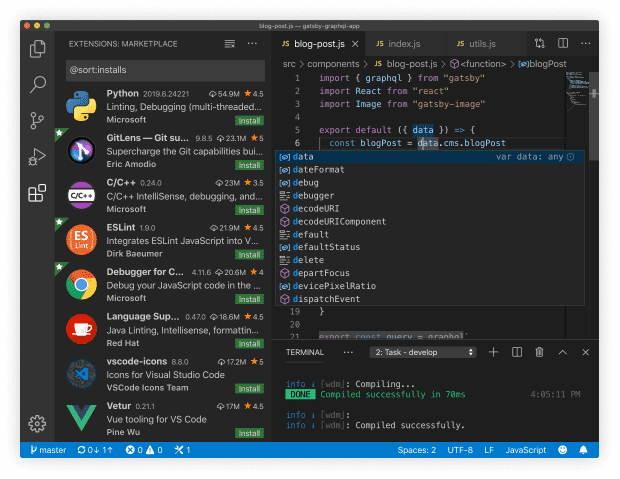
\includegraphics[width=0.9\linewidth]{graphics/home-screenshot-mac.png}	
\end{column}


\end{columns}


	
	
		
\end{frame}


\begin{frame}{Writing in python}
	\begin{enumerate}
		\item \textbf{.py files}
		
		\item \textbf{.ipynb Notebooks}
	\end{enumerate}
\end{frame}


\section{Environments}

\begin{frame}{What are environments?}
 	
\end{frame}

\begin{frame}{Virtual environments}
 	
\end{frame}




\end{document}
